\chapter{Metodologia} \label{cap:ferramentas}

O texto a seguir abordará o problema descrito neste trabalho e, logo em seguida, será apresentado um modelo de resolução utilizando algoritmos supervisionados, e mais ao final deste capítulo é realizado um exemplo de rotulação, onde será feita desde a discretição até o encontro dos rótulos para melhor explanar o contéudo descrito.

\section{Rotulação de Cluster}\label{cap:ferramentas:sec:considproblema}

A abordagem do problema referente a essa proposta de mestrado segue uma linha já pequisada que seria o \textbf{Problema de Rotulação}. Muitas pesquisas realizadas na área de rotulação fazem referência a classificação dos dados e não da rotulação. Ao agrupar um conjunto de elementos por um derterminado critério, está havendo uma classificação desses elementos de mesma similaridade, mas pouco se sabe qual é a compreensão desses grupos já classificado, no sentido de, quais os atributos são mais relevantes dentro desses grupos.

A importância do rótulo em um cluster é transparecer a compreensão do cluster formado, visto que, uma vez os clusters já agrupados não fica claro o critério de criação desses grupos. Para o observador é interessante existir um rótulo de um grupo oferecendo elementos que possam ajudar em alguma tomada de decisão em razão de seu significado, ou seja, o rótulo. Dessa forma serão apresentadas 2 (duas) definições que se complementam.

Na definição \ref{teo:problema} é expressa formalmente o comportamento dos clusters, e na definição \ref{teo:resolucao} complementa a definição \ref{teo:problema} definindo o comportamento do rótulo.

%\newtheorem{teorema}{Definição}
    \begin{teorema}
    Dado um conjunto de clusters ${C=\{c_1,...,c_k | K \geqslant 1\} }$, de modo que cada cluster contém um conjunto de elementos ${c_i=\{\vec{e}_1,..,\vec{e}_{n^{(c_i)}}|n^{(c_i)} \geqslant 1 \}}$ que podem ser representados por um vetor de atributos definidos em ${\mathbb{R}^m }$ e expresso por ${ \vec{e}^{c_i}=(a_1,..,a_m)  }$ e ainda que  com ${ c_i \cap c_{i'}=\emptyset }$ com ${ 1 \leqslant i, i \leqslant K  }$ e ${ i \neq i' }$ (Adaptada de \cite{LOPES2014}).
        %\footnotemark 
        %\footnotetext{Adaptada de \cite{LOPES2014}}
        \begin{itemize}[noitemsep]
            \item ${K}$ é o número de clusters;
            \item ${a}$ é o atributo
            \item ${c_i}$ é o i-ésimo cluster qualquer;
            \item ${n^{c_i}}$ é o número de elementos do cluster ${c_i}$;
            \item ${\vec{e}^{(c_i)}_j}$ se refere ao j-ésimo  elemento (registro na tabela) pertencente ao cluster ${c_i}$;
            \item ${m}$ é o número de atributos da tabela de dados;
        \end{itemize}
    \label{teo:problema}
    \end{teorema}

A criação do rótulo é a escolha de uma tupla \textbf{atributo} e \textbf{faixa de valor}, onde o atributo possui  o maior  valor de correlacionamento entre os outros atributos, e a faixa escolhida, uma vez com os dados já discretizados, é aquele valor que mais se repete, dentro do atributo rótulo selecionado - por exemplo, um vetor de valores já discretizados \footnote{ seção \ref{cap:refTeor:sec:discret}} , ${\vec{v}_i=\{1,1,1,2,2,2,2,3,3\}}$, sendo $i\leqslant m$ e ${(\vec{v})}$ representando todos os elementos da coluna representada pelo atributo rótulo  ${(a)}$. Neste vetor (${\vec{v}}$) o valor que mais se repete é o número 2, então, a \textbf{faixa 2} do atributo rótulo, é a escolhida para compor o rótulo. Isto posto, o rótulo é o atributo representado por ${a}$ junto com a representação da faixa 2 (dois), e podendo em outra situação, o rótulo de um cluster ser composto por mais de uma tupla: atributo,faixa. (Definição \ref{teo:problema}).



%\afterpage{
%    \begin{quotation}

%        \textit{ Dado um conjunto de clusters ${C=\{c_1,...,c_k | K \geqslant 1\} }$, de modo que cada cluster contém um conjunto de elementos ${c_i=\{\vec{e}_1,..,\vec{e}_{n^{(c_i)}}|n^{(c_i)} \geqslant 1 \}}$ que podem ser representados por um vetor de atributos definidos em ${\mathbb{R}^m }$ e expresso por ${ \vec{e}^{c_i}=(a_1,..,a_m)  }$ e ainda que  com ${ c_i \cap c_{i'}=\{0\} }$ com ${ 1 \leqslant i, i \leqslant K  }$ e ${ i \neq i' }$.
%        }\footnotemark 

%        \footnotetext{Extraída de \cite{Lopes}}
%        \begin{itemize}[noitemsep]
%            \item ${K}$ é o número de clusters;
%            \item ${c_i}$ é o i-ésimo cluster qualquer;
%            \item ${n^{c_i}}$ é o número de elementos do cluster ${c_i}$;
%            \item ${\vec{e}_{n^{(c_i)}}}$ se refere ao j-ésimo elemento pertencente ao cluster ${c_i}$;
%            \item ${m}$ é a dimensão do problema;
%        \end{itemize}
%    \end{quotation}
    %\footnotetext{Extraída de \cite{Lopes}}
%}

\section{O Modelo de Resolução}\label{cap:ferramentas:sec:modeloresolucao}

A partir da definição do problema - \textit{Definição ~\ref{teo:problema}} - um estudo  foi desenvolvido nesta pesquisa, a fim de ser possível realizar rotulação de dados com  algoritmos supervisionados com características distintas.


Este modelo de resolução consiste em apresentar como saída um conjunto de rótulos, onde cada rótulo específico é dado por um conjunto de pares de valores, atributo e seus respectivos intevalos, gerados a partir das frequências dos valores repetidos neste intervalo. Segue \textit{Definição ~\ref{teo:resolucao}} formalizando a saída do modelo:
%\newtheorem{teorema}{Definição}
    \begin{teorema}
    Dado um conjunto de rótulos ${ R=\{ r_{c1},...,r_{ck} \} }$, no qual cada rótulo específico é dado por um conjunto de pares de valores, correspondendo a um vetor com atributo e seu respectivo intervalo, ${ r_{ci}=\{ (a_1,[p_1,q_1]),...,(a_{m^{(c_i)}}, ]p_{m^{(c_i)}},q_{m^{(c_i)}}]) \} }$ capaz de melhor expressar o cluster ${c_i}$ (Adaptada de \cite{Lopes2016}).
        %\footnotemark 
        %\footnotetext{Adaptada de \cite{LOPES2014}}
        \begin{itemize}[noitemsep]
            \item ${k}$ número de rótulos;
            \item ${R}$ representa o conjunto de rótulos na saída do modelo;
            \item ${a}$ é o atributo
            \item ${c_i}$ é o i-ésimo cluster;
            \item ${r_{c_i}}$ é o rótulo referente ao cluster ${c_i}$;
            \item ${]p_{m^{(c_i)}},q_{m^{(c_i)}}]}$ representa o intervalo de valores do atributo ${a_{m^{(c_i)}} }$, onde ${ p_{m^{(c_i)}} }$  é o limite inferior e ${ q_{m^{(c_i)}} }$ é o limite superior;
            \item ${m}$ é o número de atributos da tabela de dados;
        \end{itemize}
    \label{teo:resolucao}
    \end{teorema}

Como apresentado na seção \ref{cap:refTeor:sec:trabcorrel}, o autor \cite{LOPES2014} foca em rotulação automática de grupos utilizando a estratégia de aprendizagem de máquina supervisionada, com paradigma conexionista, para realizar seu trabalho. Porém, nesta pesquisa, foi aplicado no modelo de resolução  3 (três) algoritmos supervisionados com atuações diferentes  do que já havia sido testado anteriormente, e realizando a rotulação de dados.


\begin{figure}[h!]
        \centering
        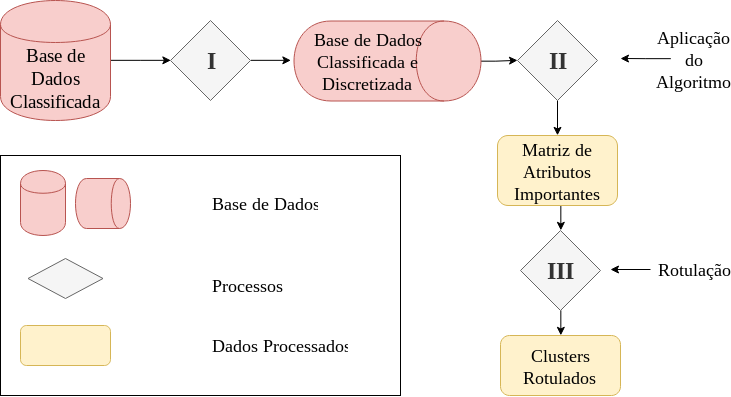
\includegraphics[scale=0.7]{figs/modeloResolucao.png}
        \caption{Modelo de Resolução Proposto} \label{fig:modeloresolucao}
\end{figure}

A base de dados\footnote{UCI - Machine Learning Repository. http://archive.ics.uci.edu/ml/} do modelo (figura \ref{fig:modeloresolucao}) conterá  valores contínuos, contudo, conforme modelo,  aplicará o método de discretização (I). Uma vez com a base discretizada ocorrerá a divisão em clusters, que nada mais é do que a separação da base em grupos já classificados mostrado na figura no fluxo ${a}$. É importante ressaltar que no fluxo ${a}$ serve para mostrar como será a entrada no passo II, pois os clusters já são definidos na própria base.

\begin{figure}[h!]
        \centering
        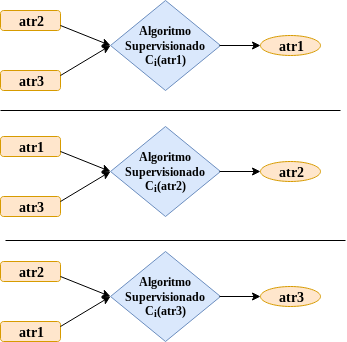
\includegraphics[scale=0.7]{figs/tecnicamodeloComp.png}
        \caption{Exemplo da técnica de correlação aplicada aos atributos atr1, atr2 e atr3. } \label{fig:tecnicamodelocomp}
\end{figure}

No passo II será executado o algoritmo de aprendizagem supervisionado, já visto nas subseções \ref{cap:refTeor:sssec:cart}, \ref{cap:refTeor:sssec:nbayes} e \ref{cap:refTeor:sssec:knn}. Essa etapa utiliza a técnica de correlação de atributos, que neste modelo de resolução é considerado o processo de maior importância, e será visto na seção  \ref{cap:ferramentas:sec:tecnica}. A  aplicação dessa técnica de correlação de atributos é exibida em um exemplo na figura \ref{fig:tecnicamodelocomp}, onde expõe o funcionamento, e o porquê do algoritmo ser executado na mesma quantidade de vezes do número de atributos, conforme uma base fictícia de 3 (três) atributos (atr1,atr2 e atr3).




A saída do processo II gera uma matriz de atributos com seus respectivos valores, e  que através desses valores armazenados é escolhido um, ou mais, atributos de maior relevância. Para gerar essa matriz conforme modelo figura \ref{fig:modeloresolucao} o algoritmo supervisionado será aplicado em uma quantidade igual ao número de atributos, ilustrado na figura \ref{fig:tecnicamodelocomp} como exemplo, onde neste caso o algoritmo supervisionado seria executado três vezes, sendo essa quantidade igual ao número de atributos: \textbf{atr1, atr2} e \textbf{atr3}.

%A quantidade de vezes que o algoritmo supervisionado é aplicado - dimensão ${m}$ da Definição \ref{teo:problema} -  irá ser a mesma do número de atributos do conjunto de dados. Utilizando a figura \ref{fig:tecnicamodelocomp} como exemplo, o algoritmo supervisionado seria executado três vezes, sendo essa quantidade igual ao número de atributos: \textbf{atr1, atr2} e \textbf{atr3}. 


Seguindo para o processo (III) acontecerá a escolha do atributo mais relevante (maior valor), e podendo, em caso de mesmo valor, ter mais de um atributo relevante. Esta seleção será feita a partir da matriz (\textbf{Atributos Importantes}) criada pela implementação dos algoritmos supervisionados utilizando a técnica de correlação entre atributos seção (\ref{cap:ferramentas:sec:tecnica}), junto com o valor mais frequente desse(s) atributo(s). Após essa etapa é criado um conjunto de rotulos para cada clusters. 

\section{Técnica de Correlação entre Atributos através de Algoritmos Supervisionados}\label{cap:ferramentas:sec:tecnica}

Essa técnica \cite{LOPES2014} utiliza por analogia a aprendizagem supervisionada, no qual os atributos de entrada são correlacionados com um atributo classe (atributo de saída). Conforme o número de atributos do cluster o atributo classe seria alterado seguindo uma sequência do primeiro ao último atributo desse cluster. Através desse processo cada atributo seria classe em relação aos outros atributos gerando um valor que seria armazenado em uma matriz.

De acordo com essa técnica os atributos de um cluster, descartando o atributo classe, seriam percorridos um por um, até o último. E a cada iteração de um atributo enquanto classe, seria armazenado o valor desse atributo em uma matriz chamada de atributos importantes. Essa matriz após montada mostraria os valores de cada atributo enquanto classe, e quanto maior o valor, mais relevante será este atributo em relação aos demais. Essa matriz é definida que em suas linhas serão armazenadas os clusters compondo a cada coluna os resultados dos atributos classe. Então caso uma base possua 2 (dois) clusters e 3 (três) atributos, a matriz seria de ordem 2x3 (2 linhas e 3 colunas).

Tal técnica possui um grau de processamento diretamente proporcional a quantidade de características expressa na base de dados definido em ${R^m}$ descrita na definição \ref{teo:resolucao}, onde ${R}$ representa o conjunto de rótulos e ${m}$ a dimensão do problema (número de atributos). Ela implica em utilizar todos os atributos, menos o definido como classe, para fazer uma correlação entre eles junto ao algoritmo.


Utilizando como exemplo uma base com os seguintes atributos: \textbf{atr1, atr2, atr3 e classe}. Retirando o atributo classe, e atribuindo a cada iteração, um  novo atributo classe, portanto,  a base possui três atributos, então o algoritmo será aplicado três vezes, um para cada atributo gerando um valor que será armazenado em uma matriz. Em um primeiro processamento de três, o primeiro atributo \textbf{atr1} se torna classe e executado com os outros dois atributos, \textbf{atr2, atr3} de entrada com um algoritmo supervisionado, figura \ref{fig:tecnicamodelo}.

\begin{figure}[h!]
        \centering
        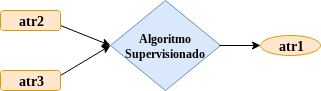
\includegraphics[scale=0.7]{figs/tecnicamodelo.png}
        \caption{Exemplo da técnica de correlação aplicada ao atributo, atr1, sendo classe } \label{fig:tecnicamodelo}
\end{figure}

O resultado da correlação entre os atributos \textbf{atr2, atr3} em relação ao \textbf{atr1} (figura \ref{fig:tecnicamodelo}) é armazanado em uma matriz, denominada de \textbf{Atributos Importantes}, de acordo com figura \ref{fig:modeloresolucao}. Por conseguinte é realizado a aplicação do algoritmo com \textbf{atr2} sendo classe, e assim sucessivamente até o último atributo (\textbf{atr3}). Essa etapa só é finalizada quando todos os atributos tiverem a chance de ser classe, coforme demonstrado na figura \ref{fig:tecnicamodelocomp}, e armazenado seus valores em porcentagem na tabela, e quanto maior sua porcentagem, mais bem correlacionado é o atributo em relação aos demais.

\section{Exemplo} \label{cap:ferramentas:sec:exebasemodfic}

Para melhor esclarecer as etapas do modelo de resolução exibido na figura \ref{fig:modeloresolucao}, será utilizado  a tabela \ref{tab:bdm} como exemplo no  modelo proposto nesta pesquisa. Essa tabela é composta por cinquenta linhas e quatro atributos, sendo o último, um atributo classe representando o cluster. Logo na primeira coluna da tabela, possui o índice da linha da tabela identificando cada registro, e outros campos são atributos que definem características do registro identificado pelo índice da primeira coluna até a quinta coluna representando a classe de cada registro.

\begin{table}[!ht]
\centering
\caption{Base de Dados Modelo}
\label{tab:bdm}
\begin{tabular}{|l|l|l|l|c|}
\hline 
 n. & atr1 & atr2 & atr3 & classe \\ \hline
1 & 2.08 & 92.11 & 22.07 & 2 \\ \hline
2 & 1.26 & 85.03 & 20.45 & 1 \\ \hline
3 & 2.00 & 108.36 & 22.68 & 2 \\ \hline
4 & 1.74 & 43.78 & 18.72 & 3 \\ \hline
5 & 1.82 & 100.20 & 23.09 & 2 \\ \hline
6 & 1.43 & 77.59 & 21.80 & 1 \\ \hline
7 & 1.53 & 44.01 & 20.98 & 3 \\ \hline
8 & 1.14 & 107.77 & 18.99 & 2 \\ \hline
9 & 1.97 & 98.00 & 22.32 & 2 \\ \hline
10 & 1.50 & 39.67 & 21.78 & 3 \\ \hline
11 & 1.74 & 55.86 & 20.31 & 3 \\ \hline
12 & 1.80 & 65.72 & 19.62 & 1 \\ \hline
13 & 1.33 & 82.01 & 19.82 & 1 \\ \hline
14 & 1.66 & 103.93 & 21.10 & 2 \\ \hline
15 & 1.42 & 66.14 & 21.61 & 1 \\ \hline
16 & 1.87 & 88.36 & 22.45 & 2 \\ \hline
17 & 1.11 & 107.82 & 19.32 & 2 \\ \hline
18 & 2.08 & 67.66 & 20.74 & 1 \\ \hline
19 & 1.85 & 82.65 & 20.35 & 1 \\ \hline
20 & 1.04 & 102.62 & 19.46 & 2 \\ \hline
21 & 1.97 & 100.37 & 21.94 & 2 \\ \hline
22 & 1.95 & 45.70 & 22.10 & 3 \\ \hline
23 & 1.77 & 50.04 & 20.16 & 3 \\ \hline
24 & 1.97 & 81.57 & 19.83 & 1 \\ \hline
25 & 1.52 & 93.13 & 20.61 & 2 \\ \hline
  \end{tabular}
  \begin{tabular}{ |l|l|l|l|c| }
   
\hline
n.  & atr1 & atr2 & atr3 & classe \\ \hline
26 & 1.42 & 53.51 & 19.64 & 3 \\ \hline
27 & 1.12 & 62.71 & 19.07 & 1 \\ \hline
28 & 2.09 & 60.58 & 20.20 & 1 \\ \hline
29 & 1.95 & 69.23 & 19.68 & 1 \\ \hline
30 & 1.03 & 47.81 & 19.47 & 3 \\ \hline
31 & 1.75 & 90.92 & 21.39 & 2 \\ \hline
32 & 1.72 & 42.35 & 22.89 & 3 \\ \hline
33 & 1.47 & 101.77 & 19.20 & 2 \\ \hline
34 & 1.53 & 41.16 & 22.67 & 3 \\ \hline
35 & 1.44 & 93.61 & 21.03 & 2 \\ \hline
36 & 1.51 & 98.65 & 19.24 & 2 \\ \hline
37 & 1.06 & 68.82 & 21.68 & 1 \\ \hline
38 & 1.48 & 80.40 & 21.43 & 1 \\ \hline
39 & 1.14 & 61.59 & 19.90 & 1 \\ \hline
40 & 1.08 & 91.93 & 20.81 & 2 \\ \hline
41 & 1.62 & 79.21 & 18.43 & 1 \\ \hline
42 & 1.68 & 80.87 & 18.42 & 1 \\ \hline
43 & 1.81 & 98.24 & 22.13 & 2 \\ \hline
44 & 1.30 & 69.27 & 18.83 & 1 \\ \hline
45 & 1.80 & 101.21 & 21.61 & 2 \\ \hline
46 & 1.79 & 72.02 & 22.02 & 1 \\ \hline
47 & 1.56 & 81.71 & 22.10 & 1 \\ \hline
48 & 1.98 & 77.16 & 21.71 & 1 \\ \hline
49 & 1.86 & 89.12 & 22.84 & 2 \\ \hline
50 & 1.55 & 76.01 & 19.74 & 1 \\ \hline
\end{tabular}
\end{table}

Seguindo a definição \ref{teo:problema} um elemento é expresso por um vetor  de dimensão ${m}$, com tamanho igual ao número de atributos. Um exemplo do elemento 2 da tabela \ref{tab:bdm}, pode ser representado por ${\vec{e}_{2}=(1.26,85.03, 20.45)}$.

\subsection{Processo (I) - Discretização} \label{cap:ferramentas:ssec:disc}

Segundo \cite{Catlett2006b,Hwang2002} através de resultados experimentais, na conversão em atributos discretos ordenados de vários domínios constatou que a mudança de representação da informação na maioria das vezes  pode aumentar a acurácia do sistema de aprendizado. Dessa maneira a etapa de discretização ganha um papel importante no modelo, e também no processo de Rotulação (III), pois é utilizada uma inferência na faixa discretizada para encontrar o intervalo na faixa.

Utilizando como exemplo a tabela \ref{tab:bdm} será utilizada a técnica de discretização por frequências iguais - EFD - e divisão de números de faixas igual a R=3. Na figura\ref{fig:EFD_R_3} poderá ser vizualizado como é feita a discretização.

 \begin{figure}[!h]
    \centering
    \subfloat[Discretização em atr1]{
        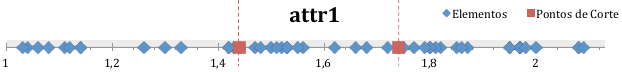
\includegraphics[scale=0.8]{figs/discretizacaoEFD_R_3_atr1.png}
        \label{fig:EFD_R_3:efd:atr1} }
    
    \subfloat[Discretização em atr2]{
        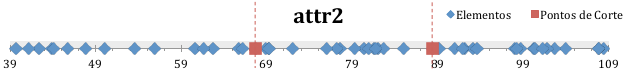
\includegraphics[scale=0.8]{figs/discretizacaoEFD_R_3_atr2.png}
        \label{fig:EFD_R_3:efd:atr2} }
    
    \subfloat[Discretização em atr3]{
        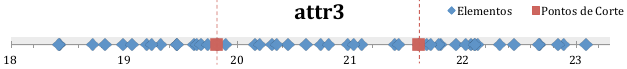
\includegraphics[scale=0.8]{figs/discretizacaoEFD_R_3_atr3.png}
        \label{fig:EFD_R_3:efd:atr2} } 
    
    \caption{Discretização de atributos utilizando EFD com R = 3 (Figura adaptada de \cite{Lopes2016})} \label{fig:EFD_R_3}
        
        %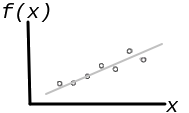
\includegraphics[scale=0.4]{figs/grafB.png}
        %\caption{Polinômio Superajustado} \label{grafB}
\end{figure}

Através da figura \ref{fig:EFD_R_3} fica claro o conteúdo da faixa 1, contendo o valor inicial, 1(um), até o primeiro ponto de corte. Na faixa 2, o valor inicial é o primeiro número após o primeiro ponto de corte (término da faixa 1) até o segundo ponto de corte, incluindo o próprio ponto de corte. E na faixa 3 contém todos  valores a partir do segundo ponto de corte.

\begin{table}[!ht]
\centering
\caption{Base de Dados Modelo Discretizada}
\label{tab:bdmd}
\begin{tabular}{|lllll|}
\hline 
  & atr1 & atr2 & atr3 & classe \\ \hline
1	&	3	&	3	&	3	&	2	\\	\hline
2	&	1	&	2	&	2	&	1	\\	\hline
3	&	3	&	3	&	3	&	2	\\	\hline
4	&	2	&	1	&	1	&	3	\\	\hline
5	&	3	&	3	&	3	&	2	\\	\hline
6	&	1	&	2	&	3	&	1	\\	\hline
7	&	2	&	1	&	2	&	3	\\	\hline
8	&	1	&	3	&	1	&	2	\\	\hline
9	&	3	&	3	&	3	&	2	\\	\hline
10	&	2	&	1	&	3	&	3	\\	\hline
11	&	2	&	1	&	2	&	3	\\	\hline
12	&	3	&	1	&	1	&	1	\\	\hline
13	&	1	&	2	&	1	&	1	\\	\hline
14	&	2	&	3	&	2	&	2	\\	\hline
15	&	1	&	1	&	2	&	1	\\	\hline
16	&	3	&	2	&	3	&	2	\\	\hline
17	&	1	&	3	&	1	&	2	\\	\hline
18	&	3	&	1	&	2	&	1	\\	\hline
19	&	3	&	2	&	2	&	1	\\	\hline
20	&	1	&	3	&	1	&	2	\\	\hline
21	&	3	&	3	&	3	&	2	\\	\hline
22	&	3	&	1	&	3	&	3	\\	\hline
23	&	3	&	1	&	2	&	3	\\	\hline
24	&	3	&	2	&	2	&	1	\\	\hline
25	&	2	&	3	&	2	&	2	\\	\hline
  \end{tabular}
  \begin{tabular}{ |lllll| }
   
\hline
  & atr1 & atr2 & atr3 & classe \\ \hline
26	&	1	&	1	&	1	&	3	\\	\hline
27	&	1	&	1	&	1	&	1	\\	\hline
28	&	3	&	1	&	2	&	1	\\	\hline
29	&	3	&	2	&	1	&	1	\\	\hline
30	&	1	&	1	&	1	&	3	\\	\hline
31	&	3	&	3	&	2	&	2	\\	\hline
32	&	2	&	1	&	3	&	3	\\	\hline
33	&	2	&	3	&	1	&	2	\\	\hline
34	&	2	&	1	&	3	&	3	\\	\hline
35	&	1	&	3	&	2	&	2	\\	\hline
36	&	2	&	3	&	1	&	2	\\	\hline
37	&	1	&	2	&	3	&	1	\\	\hline
38	&	2	&	2	&	2	&	1	\\	\hline
39	&	1	&	1	&	2	&	1	\\	\hline
40	&	1	&	3	&	2	&	2	\\	\hline
41	&	2	&	2	&	1	&	1	\\	\hline
42	&	2	&	2	&	1	&	1	\\	\hline
43	&	3	&	3	&	3	&	2	\\	\hline
44	&	1	&	2	&	1	&	1	\\	\hline
45	&	3	&	3	&	2	&	2	\\	\hline
46	&	3	&	2	&	3	&	1	\\	\hline
47	&	2	&	2	&	3	&	1	\\	\hline
48	&	3	&	2	&	3	&	1	\\	\hline
49	&	3	&	3	&	3	&	2	\\	\hline
50	&	2	&	2	&	1	&	1	\\	\hline

\end{tabular}
\end{table}

A tabela \ref{tab:bdmd} é o resultado após a discretização de todos os atributos. Para cada base de dados será definido o número de faixas de acordo com a configuração inicial antes da execução. Nessa configuração do sistema o número de faixas serve para toda a base de dados e não para cada atributo, então nesse exemplo o valor de ${R=3}$ conforme figura \ref{fig:EFD_R_3}, onde ${R}$ é o número de faixas a ser dividido tanto no \textbf{atr1} como também no \textbf{atr2} e \textbf{atr3} possuem os valores conforme tabela \ref{tab:faixas}.

% Please add the following required packages to your document preamble:
% \usepackage[table,xcdraw]{xcolor}
% If you use beamer only pass "xcolor=table" option, i.e. \documentclass[xcolor=table]{beamer}
\begin{table}[]
\centering
\caption{Valores das faixas com R=3 da Base de Dados Modelo}
\label{tab:faixas}
\begin{tabular}{lrrr}
\rowcolor[HTML]{C0C0C0} 
                                     & \multicolumn{1}{c}{\cellcolor[HTML]{C0C0C0}\textbf{Faixa 1}} & \multicolumn{1}{c}{\cellcolor[HTML]{C0C0C0}\textbf{Faixa 2}} & \multicolumn{1}{c}{\cellcolor[HTML]{C0C0C0}\textbf{Faixa 3}} \\
\rowcolor[HTML]{FFFFFF} 
{\color[HTML]{333333} \textbf{atr1}} & {[} 1.03 $\sim$1.44 {]}                                      & {]} 1.44 $\sim$1.74 {]}                                      & {]} 1.74 $\sim$2.09 {]}                                      \\
\rowcolor[HTML]{EFEFEF} 
{\color[HTML]{000000} \textbf{atr2}} & {\color[HTML]{000000} {[} 39.67 $\sim$67.66 {]}}             & {\color[HTML]{000000} {]} 67.66 $\sim$88.36 {]}}             & {\color[HTML]{000000} {]} 88.36 $\sim$108.36 {]}}            \\
\rowcolor[HTML]{FFFFFF} 
\textbf{atr3}                        & {[} 18.42 $\sim$19.82 {]}                                    & {]} 19.82 $\sim$21.61 {]}                                    & {]} 21.61 $\sim$23.09 {]}                                   
\end{tabular}
\end{table}

% Conforme cada valor discreto representando um intervalo, poderá o algoritmo está perdendo um pouco de informação, pois a discretização acaba generalizando a informação por agrupar os dados em intervalos representando-os de forma mais igual. Mas um fato a se levar em consideração é o número de faixas de valores, de uma variável discreta, pois se esse número for muito grande poderá acarretar ausência de generalização.


\subsection{Processo (II) - Algoritmos Supervisionados}\label{cap:ferramentas:ssec:algsuper}

Ao chegar nessa etapa, Processo (II) da figura \ref{fig:modeloresolucao}, já se tem uma base discretizada e clusters formados como visto na tabela \ref{tab:bdmd}. A partir desta etapa é feita a execução do algorimo de aprendizado supervisionado obtendo como saída um valor, em porcentagem, informando o grau de correlacionamento entre os atributos compondo  uma matriz, cuja função é armazenar o resultado da execução dos algoritmos utilizando a técnica de correlação de atributos (\ref{cap:ferramentas:sec:tecnica}).

O algoritmo irá selecionar cluster por cluster, percorrendo todos os atributos destes clusters, onde a cada iteração um atributo será a classe da vez. Nesse exemplo, primeiramente o atributo \textbf{atr1} será classe e os demais irão participar como entrada junto ao algoritmo, verificando seu grau de importância entre eles. Depois o atributo \textbf{atr2} irá ser classe, e depois o \textbf{atr3}, fechando o ciclo de todos os atributos do cluster, visualizado na figura \ref{fig:tecnicamodelocomp}.
% \begin{figure}[h!]
%         \centering
%         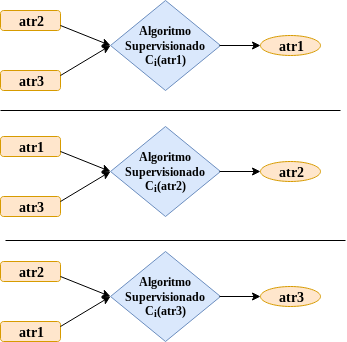
\includegraphics[scale=0.7]{figs/tecnicamodeloComp.png}
%         \caption{Exemplo da técnica de correlação aplicada aos ${3 (três)}$ atributos, cada um sendo classe em determinada iteração } \label{fig:tecnicamodelocomp}
% \end{figure}



 \begin{figure}[h!]
    \centering
    \subfloat[Execução do Naive Bayes]{
        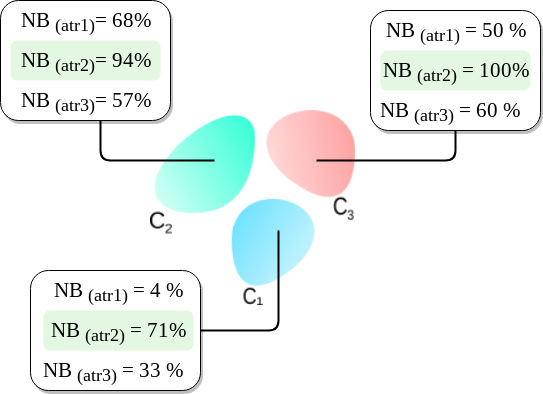
\includegraphics[scale=0.3]{figs/rotulacaoNB.png}
        \label{fig:rotulacao:rotNB} }
    \quad
    \subfloat[Execução do algorimo de Árvore de Decisão]{
        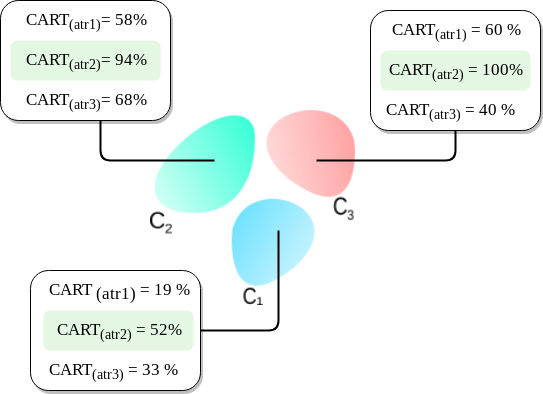
\includegraphics[scale=0.3]{figs/rotulacaoDecisionTree.png}
        \label{fig:rotulacao:rotDT} } 
    
    \caption{Resultado dos Algoritmos} \label{fig:rotulacao}
        %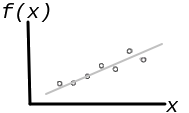
\includegraphics[scale=0.4]{figs/grafB.png}
        %\caption{Polinômio Superajustado} \label{grafB}
\end{figure}

A figura \ref{fig:rotulacao:rotNB} mostra o resultado da execução do Naive Bayes trabalhando com a base modelo (tabela \ref{tab:bdmd}) exibindo os resultados em porcentagem de acerto de cada atributo em relação aos demais. O mesmo acontece com a figura \ref{fig:rotulacao:rotDT} onde é aplicado um algorimo de Árvore de Decisão - CART - exibindo o resultado de todas as taxas de acerto, em porcentagem, dos atributos de seus respectivos clusters.

Uma forma de eliminar uma possível ambiguidade entre os clusters foi adicionar na implementação uma variável  ${V}$. Essa variável é utilizada para seleção dos atributos rótulos de um clusters, caso aconteça dos rótulos se repetirem em clusters diferentes. Logo, todos os atributos que tiverem até uma diferença ${V}$ em relação ao atributo de maior taxa de acerto, expresso em porcentagem, serão escolhidos como rótulo. Isto posto, se o atributo de maior taxa de acerto possuir ${90\%}$, e o ${V=10\%}$  então todos outros atributos que tiverem valores a partir de ${80\%}$ são selecionados como rótulo do cluster.  

O valor da variável ${V}$ é subjetivo e irá ser arbitrado de acordo com os resultados em cada aplicação do algoritmo em um conjunto de dados. Nesse exemplo caso fosse utilizado a variância ${V=12}$ na matriz de atributos importantes representada pela figura \ref{fig:rotulacao:rotNB}, teriam os atributos, por clusters, ${r_{c_i}}$ : ${r_{c_1}=\{atr2\}}$, ${r_{c_2}=\{atr2\}}$, ${r_{c_3}=\{atr2\}}$.

%O valor da variável \textbf{V} é subjetivo e irá ser arbitrado de acordo com os resultados em cada aplicação do algoritmo em cima de um conjunto de dados. Nesse exemplo caso fosse utilizado a variância \textbf{V} = 12 na matriz de atributos importantes representada pela figura \ref{fig:rotulacao:rotNB}, teriam os atributos, por clusters, r_(ci) : rc1 = \{atr2\}, rc2 = \{atr2\}, rc3 = \{atr2\}.


\subsection{Processo (III) - Rotulação} \label{cap:ferramentas:ssec:rotulacao}

No processo de rotulação os rótulos de cada cluster (${c_i}$) serão compostos conforme o  equação \ref{eq:rotulo}. 
\begin{equation}\label{eq:rotulo}
r_{ci}=\{ (a_1,[p_1,q_1]),...,(a_{m^{(c_i)}}, ]p_{m^{(c_i)}},q_{m^{(c_i)}}]) \} 
\end{equation}

 Cada rótulo é composto pela tupla:  atributo de maior relevância (matriz de atributos importantes) e a faixa de valor desse atributo que mais se repete. Na figura \ref{fig:rotulacao} os rótulos em destaque são os que possuem maior valor, ademais, cada atributo que faz parte do rótulo possui um vetor de valores, de onde será escolhido a faixa de maior ocorrência. Uma vez calculado e definido a faixa, será determinado os limites inferiores (${p_{m^{(c_i)}}}$) e superiores (${q_{m^{(c_i)}}}$) de acordo com a tabela discretizada (exemplo \ref{tab:faixas}). 


Por exemplo, utilizando a Base Modelo, mais especificamente o cluster 1 ($c_1$), cujo resultado é apresentado na figura \ref{fig:rotulacao:rotNB}, o rótulo apresentado é o atributo  \textbf{atr2} com a \textbf{faixa 2}, faixa esta encontrada após cálculo dos elementos de maior ocorrência, conforme descrito no parágrafo acima. 

O rótulo apresentado ao final do processo terá a substituição do número da faixa pelos valores do intervalo conforme a tabela \ref{tab:faixas}. Os rótulos dos clusters descrito neste exemplo - conforme figura \ref{fig:rotulacao:rotNB} e figura  \ref{fig:rotulacao:rotDT} - aplicado na BD Modelo são:

\begin{itemize}[noitemsep]
            \item ${r_{c_1}=(atr2,]67.66, 88.36])}$;
            \item ${r_{c_2}=(atr2,]88.36, 108.36])}$ ;
            \item ${r_{c_3}=(atr2,[39.67, 67.66])}$;
            
\end{itemize}

A representação acima do rótulo informa que no rótulo do cluster 1 é uma tupla composta pelo atributo, \textbf{atr2}, e a faixa variando de valor maior que 67,66 até 88,36. No cluster 2 possui o rótulo composto também pelo atributo \textbf{atr2}, mas com faixa diferente, variando de um valor maior que 88,67 até 108,36. E por último o rótulo do cluster 3 com a faixa variando de 39,67 até 67,66. Isso significa que qualquer registro com valor no atr2 no intervalo ${]67.66, 88.36]}$, será agrupado no cluster 1, podendo ajudar um analista a interpretar ou tomar decisão em conformidade a esse rótulo. Então, caso esse atr2 fosse localização e esse intervalo determinasse uma região, isso poderia ser utilizado para tomada de decisão, dependendo do problema que queira resolver.

% Uma vez terminado o processo (III) de rotulação, o fluxo ${b}$ da figura \ref{fig:modeloresolucao}, só será executado caso seja necessário  testar outro algoritmo.


O algoritmo \ref{alg:rotulacao} exibe a rotina em forma de pseudocódigo para melhor entendimento, mas as variáveis ${V}$, ${R}$ e ${TipoDiscretização}$, não foram inicializadas por serem variáveis que dependem de testes para melhor otimização dos rótulos. No caso da variância ${V}$ por padrão é inicializada com 0 (zero), porque ela é utilizada caso haja empate nos valores da matriz de importância na escolha dos rótulos, e caso assuma outro valor, ela dependerá dos valores da matriz. A variável ${R}$ é utilizada para definir em quantas faixas será dividido os valores do atributo na discretização, e por fim a variável ${TipoDiscretização}$ que também dependerá do comportamento dos valores do atributo. 

\IncMargin{1em}
\begin{algorithm}[h]

\nl $Carrega\_valores\_auxiliares(V,R,TipoDiscretização)$\;
\nl $Carrega\_BD$\; 
\nl $Discretiza\_BD$\; 
\nl $Separa\_em\_clusters\_de\_acordo\_com\_classificação\_BD$\; 
\nl \While{existir clusters}{
 \nl \While{existir atributos}{ 
      \nl $atributo\_classe$=$seleciona\_nova\_classe(atributos)$ \; 
      \nl $Aplica\_algoritmo\_supervisionado(atributo\_classe,atributos\_naoClasse)$\;
      \nl $Calcula\_matriz\_de\_porcentagem\_de\_acertos$\; 
      } 
    \nl \If{V!=0}{
        \nl $Carrega\_atributos\_importantes\_considerando\_V$\;
        }
    \nl $Associa\_valores\_aos\_intervalos$\; 
 }
 \nl $Exibe\_rótulos\_todos\_clusters$\; 
 \caption{Rotina de Rotulação}\label{alg:rotulacao}
 
\end{algorithm}
\DecMargin{1em}
        
